% Options for packages loaded elsewhere
\PassOptionsToPackage{unicode}{hyperref}
\PassOptionsToPackage{hyphens}{url}
%
\documentclass[
]{article}
\usepackage{lmodern}
\usepackage{amssymb,amsmath}
\usepackage{ifxetex,ifluatex}
\ifnum 0\ifxetex 1\fi\ifluatex 1\fi=0 % if pdftex
  \usepackage[T1]{fontenc}
  \usepackage[utf8]{inputenc}
  \usepackage{textcomp} % provide euro and other symbols
\else % if luatex or xetex
  \usepackage{unicode-math}
  \defaultfontfeatures{Scale=MatchLowercase}
  \defaultfontfeatures[\rmfamily]{Ligatures=TeX,Scale=1}
\fi
% Use upquote if available, for straight quotes in verbatim environments
\IfFileExists{upquote.sty}{\usepackage{upquote}}{}
\IfFileExists{microtype.sty}{% use microtype if available
  \usepackage[]{microtype}
  \UseMicrotypeSet[protrusion]{basicmath} % disable protrusion for tt fonts
}{}
\makeatletter
\@ifundefined{KOMAClassName}{% if non-KOMA class
  \IfFileExists{parskip.sty}{%
    \usepackage{parskip}
  }{% else
    \setlength{\parindent}{0pt}
    \setlength{\parskip}{6pt plus 2pt minus 1pt}}
}{% if KOMA class
  \KOMAoptions{parskip=half}}
\makeatother
\usepackage{xcolor}
\IfFileExists{xurl.sty}{\usepackage{xurl}}{} % add URL line breaks if available
\IfFileExists{bookmark.sty}{\usepackage{bookmark}}{\usepackage{hyperref}}
\hypersetup{
  pdftitle={Supervised Machine Learning HW 5},
  pdfauthor={Group 3: Maja Nordfeldt, Jakob Rauch, Timo Schenk, Konstantin Sommer},
  hidelinks,
  pdfcreator={LaTeX via pandoc}}
\urlstyle{same} % disable monospaced font for URLs
\usepackage[margin=1in]{geometry}
\usepackage{color}
\usepackage{fancyvrb}
\newcommand{\VerbBar}{|}
\newcommand{\VERB}{\Verb[commandchars=\\\{\}]}
\DefineVerbatimEnvironment{Highlighting}{Verbatim}{commandchars=\\\{\}}
% Add ',fontsize=\small' for more characters per line
\usepackage{framed}
\definecolor{shadecolor}{RGB}{248,248,248}
\newenvironment{Shaded}{\begin{snugshade}}{\end{snugshade}}
\newcommand{\AlertTok}[1]{\textcolor[rgb]{0.94,0.16,0.16}{#1}}
\newcommand{\AnnotationTok}[1]{\textcolor[rgb]{0.56,0.35,0.01}{\textbf{\textit{#1}}}}
\newcommand{\AttributeTok}[1]{\textcolor[rgb]{0.77,0.63,0.00}{#1}}
\newcommand{\BaseNTok}[1]{\textcolor[rgb]{0.00,0.00,0.81}{#1}}
\newcommand{\BuiltInTok}[1]{#1}
\newcommand{\CharTok}[1]{\textcolor[rgb]{0.31,0.60,0.02}{#1}}
\newcommand{\CommentTok}[1]{\textcolor[rgb]{0.56,0.35,0.01}{\textit{#1}}}
\newcommand{\CommentVarTok}[1]{\textcolor[rgb]{0.56,0.35,0.01}{\textbf{\textit{#1}}}}
\newcommand{\ConstantTok}[1]{\textcolor[rgb]{0.00,0.00,0.00}{#1}}
\newcommand{\ControlFlowTok}[1]{\textcolor[rgb]{0.13,0.29,0.53}{\textbf{#1}}}
\newcommand{\DataTypeTok}[1]{\textcolor[rgb]{0.13,0.29,0.53}{#1}}
\newcommand{\DecValTok}[1]{\textcolor[rgb]{0.00,0.00,0.81}{#1}}
\newcommand{\DocumentationTok}[1]{\textcolor[rgb]{0.56,0.35,0.01}{\textbf{\textit{#1}}}}
\newcommand{\ErrorTok}[1]{\textcolor[rgb]{0.64,0.00,0.00}{\textbf{#1}}}
\newcommand{\ExtensionTok}[1]{#1}
\newcommand{\FloatTok}[1]{\textcolor[rgb]{0.00,0.00,0.81}{#1}}
\newcommand{\FunctionTok}[1]{\textcolor[rgb]{0.00,0.00,0.00}{#1}}
\newcommand{\ImportTok}[1]{#1}
\newcommand{\InformationTok}[1]{\textcolor[rgb]{0.56,0.35,0.01}{\textbf{\textit{#1}}}}
\newcommand{\KeywordTok}[1]{\textcolor[rgb]{0.13,0.29,0.53}{\textbf{#1}}}
\newcommand{\NormalTok}[1]{#1}
\newcommand{\OperatorTok}[1]{\textcolor[rgb]{0.81,0.36,0.00}{\textbf{#1}}}
\newcommand{\OtherTok}[1]{\textcolor[rgb]{0.56,0.35,0.01}{#1}}
\newcommand{\PreprocessorTok}[1]{\textcolor[rgb]{0.56,0.35,0.01}{\textit{#1}}}
\newcommand{\RegionMarkerTok}[1]{#1}
\newcommand{\SpecialCharTok}[1]{\textcolor[rgb]{0.00,0.00,0.00}{#1}}
\newcommand{\SpecialStringTok}[1]{\textcolor[rgb]{0.31,0.60,0.02}{#1}}
\newcommand{\StringTok}[1]{\textcolor[rgb]{0.31,0.60,0.02}{#1}}
\newcommand{\VariableTok}[1]{\textcolor[rgb]{0.00,0.00,0.00}{#1}}
\newcommand{\VerbatimStringTok}[1]{\textcolor[rgb]{0.31,0.60,0.02}{#1}}
\newcommand{\WarningTok}[1]{\textcolor[rgb]{0.56,0.35,0.01}{\textbf{\textit{#1}}}}
\usepackage{longtable,booktabs}
% Correct order of tables after \paragraph or \subparagraph
\usepackage{etoolbox}
\makeatletter
\patchcmd\longtable{\par}{\if@noskipsec\mbox{}\fi\par}{}{}
\makeatother
% Allow footnotes in longtable head/foot
\IfFileExists{footnotehyper.sty}{\usepackage{footnotehyper}}{\usepackage{footnote}}
\makesavenoteenv{longtable}
\usepackage{graphicx,grffile}
\makeatletter
\def\maxwidth{\ifdim\Gin@nat@width>\linewidth\linewidth\else\Gin@nat@width\fi}
\def\maxheight{\ifdim\Gin@nat@height>\textheight\textheight\else\Gin@nat@height\fi}
\makeatother
% Scale images if necessary, so that they will not overflow the page
% margins by default, and it is still possible to overwrite the defaults
% using explicit options in \includegraphics[width, height, ...]{}
\setkeys{Gin}{width=\maxwidth,height=\maxheight,keepaspectratio}
% Set default figure placement to htbp
\makeatletter
\def\fps@figure{htbp}
\makeatother
\setlength{\emergencystretch}{3em} % prevent overfull lines
\providecommand{\tightlist}{%
  \setlength{\itemsep}{0pt}\setlength{\parskip}{0pt}}
\setcounter{secnumdepth}{-\maxdimen} % remove section numbering

\title{Supervised Machine Learning HW 5}
\author{Group 3: Maja Nordfeldt, Jakob Rauch, Timo Schenk, Konstantin Sommer}
\date{25-1-2020}

\begin{document}
\maketitle

\hypertarget{introduction}{%
\section{Introduction}\label{introduction}}

Is it possible to before its screening predict whether a movie will be a
blockbuster, only based on publicly available information? This question
can be of high relevance for movie producers or producing companies that
face the issue of how to optimally plan a movies market rollout, as well
as assess the prospects of their future outcome. For example if one can
predict that a movie is likely to be a huge success one might try to
push it in more countries than only in the local one and might even
increase marketing budgets in order to gain the full potential out of
the success. Another stakeholder that might be interested are movie
theaters that might base their scheduling (room size, screening times
etc.) on it. We will analyze this question from a very neutral
perspective, without even assessing the movie quality, but only the
information that is publicly available before a movie start, which might
also be the information that decision makers will base their decision
on, especially if they are outside of the production itself (like movie
theaters).

\hypertarget{data}{%
\section{Data}\label{data}}

In order to answer our proposed question of how to predict a movie
success we are using a sample out of data published by the Internet
Movie Database (IMDb) that is publicly available for download. IMDb is
an online database, in which users can not only view information about
movies and actors/actresses but can also rank the movies. The available
datasets comprises information on movie names, director and actors as
well as on the used budget and the assigned genre of the movie. We
define a movie as being successful if it manages to gain more than three
times in box gross revenue than the available budget in the movie
production. Box gross revenue is the income a movie gains from movie
theater screenings. For both measures we are using inflation corrected
numbers in 2015 dollars and define \(gross_{x3}\) to be TRUE if the
movie was successful according to our criterium. We exclude the names of
the participating actors due to the otherwise extensive number of
categorical variables but use the number of Facebook likes of the main
actors as a proxy for the popularity of the cast and do the same for the
director of the movie. We exclude reviews from critics and IMDb users,
since they are likely to only be available after the start of the movie.
We nevertheless include the MPAA rating that gives a recommendation on
the age of the targeted audience that should be allowed to watch it
since one can expect that this might have an influence on the success of
a movie. The rating system is giving recommendations from suggested for
the general audience to only suggested for people above the age of 17.
We drop the year variable since it should be without interest for
decision makers since they can not influence the timing of the movie
release or put differently it is without interest to know if movies were
especially successful in a certain year. We additionally include 0 or 1
dummies for all genres, since movies can also fall into several of the
categories. We also include the length of the title since one can assume
that short titles might be catchier and therefore more successful.
Finally we also include the movie budget but exclude all movies with a
budget below one million dollar. A first inspection of the data shows
that their are missing values in some of the observations, which we will
drop in our manual estimation. Another important feature of the data is
its unbalanced ness. Looking at FIGURE XYZ in which we plot the movie
budget versus the movie success one can see that there is a large amount
of movies that do not make the threshold and only very few (about one
fifth) that are categorized as successful. One can also see that there
is only a few very expensive movies while most movies are in the bottom
of the budget range.

\begin{figure}[h]

{\centering 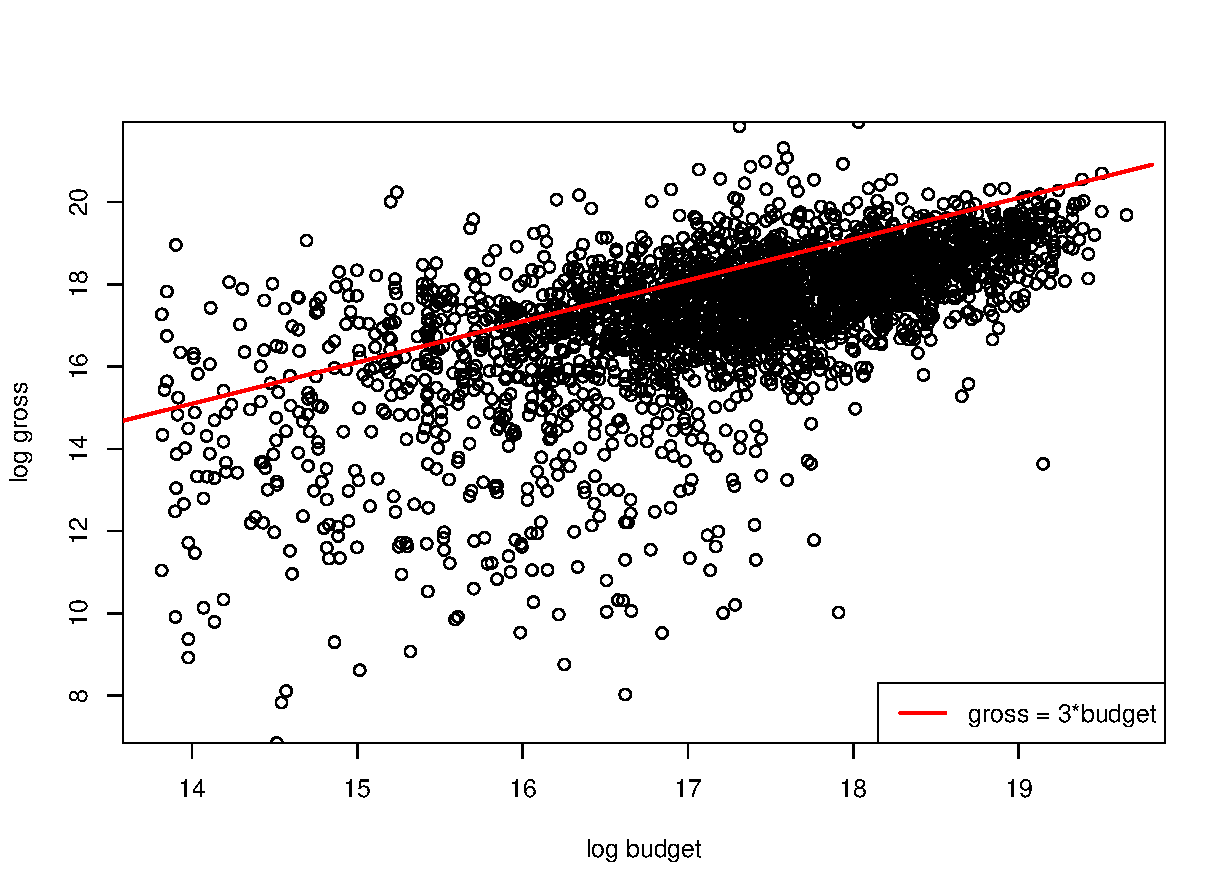
\includegraphics[width=0.5\linewidth]{./datavisual} 

}

\caption{Gross vs. Budget, logarithmed}\label{fig:unnamed-chunk-3}
\end{figure}

\hypertarget{leave-gross_2015-saved-as-separate-variable-to-get-mean-for-table}{%
\subsubsection{Leave gross\_2015 saved as separate variable to get mean
for
table}\label{leave-gross_2015-saved-as-separate-variable-to-get-mean-for-table}}

\begin{longtable}[]{@{}lccccc@{}}
\toprule
\begin{minipage}[b]{0.08\columnwidth}\raggedright
\strut
\end{minipage} & \begin{minipage}[b]{0.12\columnwidth}\centering
Budget\strut
\end{minipage} & \begin{minipage}[b]{0.12\columnwidth}\centering
Revenue\strut
\end{minipage} & \begin{minipage}[b]{0.18\columnwidth}\centering
Cast-FB-likes\strut
\end{minipage} & \begin{minipage}[b]{0.22\columnwidth}\centering
Director-FB-likes\strut
\end{minipage} & \begin{minipage}[b]{0.12\columnwidth}\centering
Duration\strut
\end{minipage}\tabularnewline
\midrule
\endhead
\begin{minipage}[t]{0.08\columnwidth}\raggedright
mean\strut
\end{minipage} & \begin{minipage}[t]{0.12\columnwidth}\centering
51619313\strut
\end{minipage} & \begin{minipage}[t]{0.12\columnwidth}\centering
84120426\strut
\end{minipage} & \begin{minipage}[t]{0.18\columnwidth}\centering
12427\strut
\end{minipage} & \begin{minipage}[t]{0.22\columnwidth}\centering
946\strut
\end{minipage} & \begin{minipage}[t]{0.12\columnwidth}\centering
110\strut
\end{minipage}\tabularnewline
\bottomrule
\end{longtable}

In table \ref(tab:1) one can see the mean of our main variables of
interest, excluding the genre dummies. One can see that the average
movie budget is 51 million 2015-US dollar, the average facebook likes of
the cast are 12 thousand and the avergae duration is 110 minutes, so 20
minutes more than the standard 90 minutes movie framework.

\hypertarget{methods}{%
\section{Methods}\label{methods}}

The predictive model we employ is a decision tree, which is found using
a greedy, recursive, divide-and-conquer algorithm. The method is best
explained using figure 1, a graph of a decision tree. For our binary
classification problem, the decision tree will consist of a number of
nodes (1,2,3,4,5,6,7). At each internal node (1,3,5), the data is split
into two parts, creating two new branches. At the terminal nodes (also
called leafs; here 2,4,6,7), we simply make our prediction as the
majority class for all observations left at the leaf: FALSE at nodes
2,4, and 6; TRUE at node 7.

We let the splitting function depend only on one variable and choose the
splitting variable and the threshold value to minimize resulting node
impurity, a function of the the share of mis-classified observations
using the splitting rule. There are different measures for node
impurity, the one we will be using in practice is the Gini impurity
given by \(G=1-p_0^2-p_1^2\), where \(p_0\) and \(p_1\) are the shares
of class FALSE and TRUE, respectively. In practice, we start at node 1
with the full dataset, try each combination of splitting variable and
threshold value (if numerical
\footnote{If categorical, we try as splitting rules all combinations of categories.})
and choose the one that results in the lowest impurity. In this case,
the best resulting splitting rule was to split movies according to
whether their budget was higher or larger than 36 million USD. We then
create two child nodes (2 and 3), at which we repeat the process of
trying to find the best splitting rule.

Following this algorithm, the tree would grow and become more specific
until many leafs contain only one observation. This would be
over-fitting, as the tree is not able to separate the noise from the
signal, and such a tree would perform very poorly out of sample. For
this reason, we need to specify a stopping rule for the tree. Popular
stopping rules include setting a maximum depth (depth is the longest
distance from the root to a leaf, here 3), or a minimum number of
observations in a node for a split to be attempted. Another approach is
to stop splitting when the resulting reduction in prediction errors
drops below a threshold. The issue with this approach is that there
might be splits which are not valuable in themselves, but that enable
valuable splits further down the line. The danger is therefore that we
stop splitting prematurely.

This can be solved with a procedure known as pruning: we fist grow a
large (overfitting) tree and then prune the large tree by removing
subtrees (such as the one starting at node 5). Specifically, we have a
pruning criterion function that is the sum of the prediction error and a
penalty \(\alpha\) on the size of the tree (the size is the number of
leafs, here 4). As \(\alpha\) increases, we will remove more and more
subtrees and end up with a lean tree with better out-of-sample
performance. As \(\alpha\) tends to infinity we end up classifying all
observations as the majority class. The optimal \(\alpha\) can be found
via k-fold cross-validation: we randomly shuffle the data and divide it
into \(k\) bins. We then use the \(k-1\) bins for training and the
remaining bin for testing out-of-sample performance, iterating \(k\)
times to use each bin as a test sample once. The optimal \(\alpha\) is
the one that gives the lowest average out-of-sample prediction error.

Another approach to get predictions from decision trees with good
out-of-sample performance is to use an ensemble of trees. A set of
training data leads to a unique optimal tree given the stopping
criteria. However, we can generate different training sets from our
existing data using by bootstrapping: if our original sample has \(n\)
observations, sampling \(n\) times with replacement from the original
sample leads to a new data set. We can create \(B\) such new samples
from \(B\) bootstraps, which will lead to \(B\) trees. Finally, we take
the `average' prediction of our tree ensemble (forest). In a binary
classification setting, the prediction for a given observation will
simply be that made by the majority of trees. This procedure is known as
bagging (= bootstrap aggregating) and makes our prediction more robust
(to the fact that our observations are noisy and we have a random
sample). Unfortunately, we lose the easily interpretable nature of a
single decision tree (as the one in figure 1) as we now have \(B\)
different trees. However, we can get a measure of which variables are
important by looking at the total decrease in Gini impurities from
splitting on the variable, averaged over all trees. Note that bagging
still requires a stopping criterion for the trees to not grow too large;
we will simply use a maximum depth.

\hypertarget{results}{%
\section{Results}\label{results}}

\hypertarget{single-tree}{%
\subsection{single tree}\label{single-tree}}

\begin{longtable}[]{@{}lrrr@{}}
\toprule
& pred 0 & pred 1 & class.error\tabularnewline
\midrule
\endhead
obs 0 & 2336 & 15 & 0.0063803\tabularnewline
obs 1 & 450 & 53 & 0.8946322\tabularnewline
\bottomrule
\end{longtable}

\begin{figure}[h]

{\centering 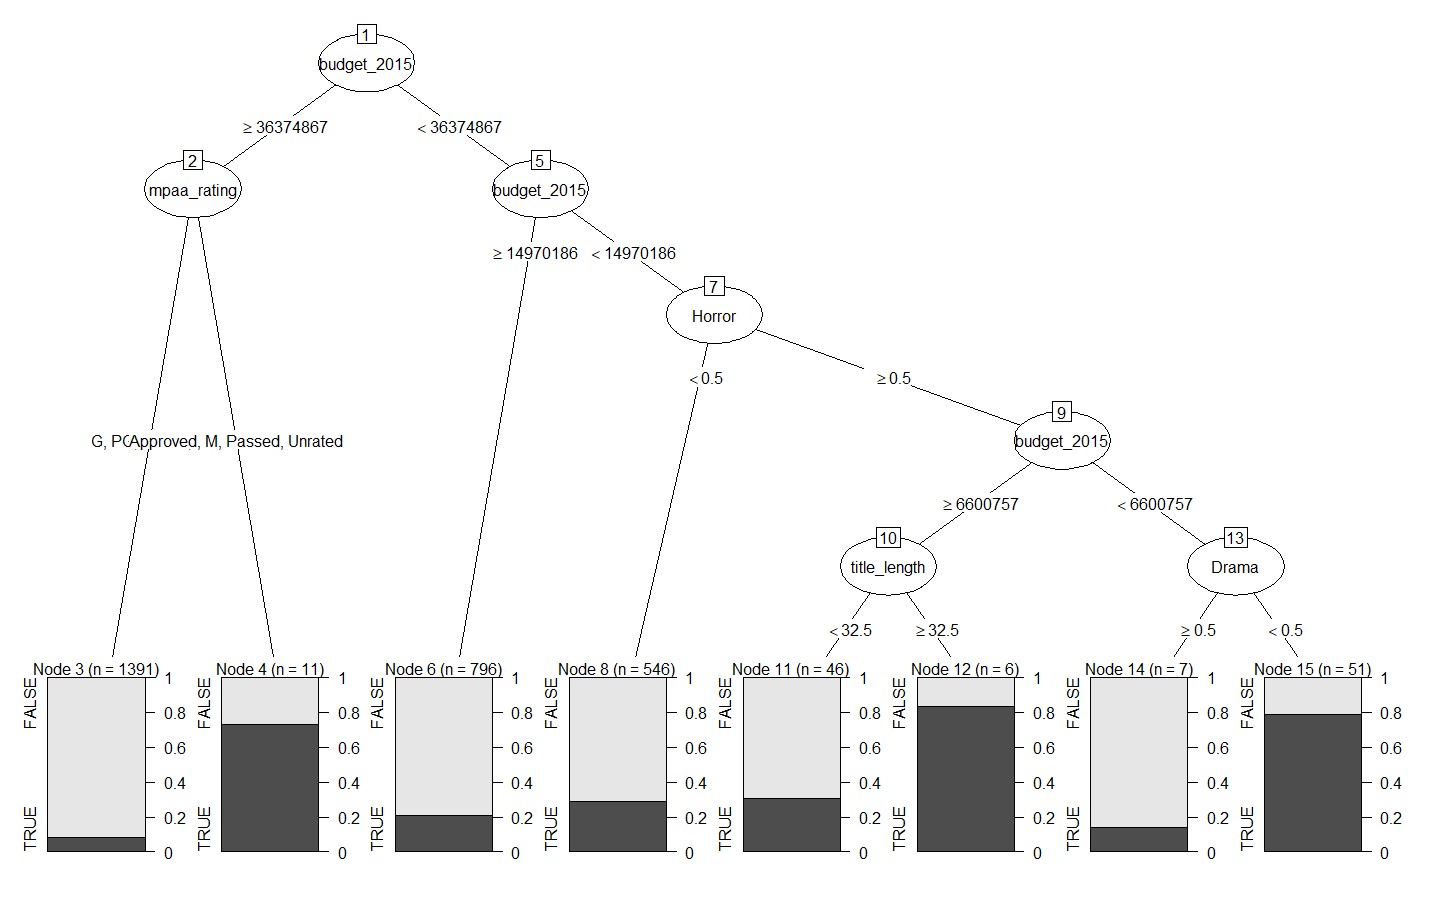
\includegraphics{./bigtree} 

}

\caption{Decision for optimal cp}\label{fig:unnamed-chunk-8}
\end{figure}

\hypertarget{bagging}{%
\subsection{bagging}\label{bagging}}

\begin{longtable}[]{@{}lrrr@{}}
\toprule
& pred 0 & pred 1 & class.error\tabularnewline
\midrule
\endhead
obs 0 & 2256 & 95 & 0.0404083\tabularnewline
obs 1 & 398 & 105 & 0.7912525\tabularnewline
\bottomrule
\end{longtable}

\begin{figure}

{\centering 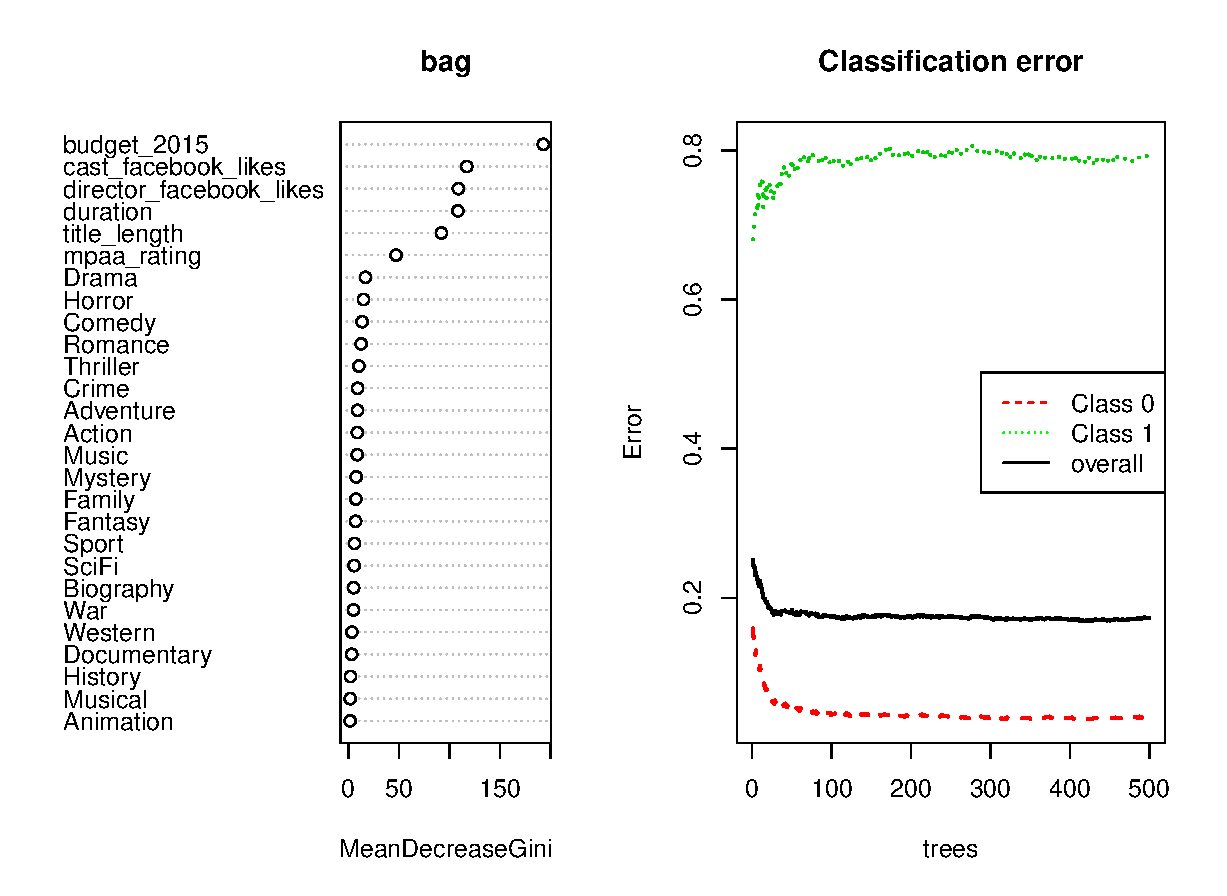
\includegraphics{./bagplots} 

}

\caption{Results bagging}\label{fig:unnamed-chunk-10}
\end{figure}

\hypertarget{conclusion-discussion}{%
\section{Conclusion \& Discussion}\label{conclusion-discussion}}

In this study, we asked the question whether we could predict whether a
produced movie would return three times its budget before the start of
its screening. Using binary classification, as well as bagging we found
that it is indeed possible.

XXX discussion of results XXXX

From a perspective of practice implementation the classification tree is
intuitive and easy to interpret, which may be a benefit if to be used
for convincing stakeholders and making collective decisions in an
organization. We can further clearly follow the steps behind the
outcome, more transparent than the ``black-box'' results of some other
methods. Data preparation needed is also sparse - variable
standardization is not needed, missing values are treated robustly and
dummies are not necessarily required for categorical variables. One also
does not need to perform feature selection as it is done implicitly, and
interactions and non-linearity is handled. On the downside, the results
may not be robust - minor changes to training data can alter tree and
final predictions, and overfitting can be a serious problem. The
usefulness of predictions in practice can therefore come into question
and results are sensitive to the quality of data.

The bagged approach help reduce variance of the traditional
classification tree, and out of bag estimates are easy to use for
validation. Although we still have easily interpretable diagnostics like
the Gini index, contrasting the classification tree we now lack the
intuitive visual interpretation. We have not included an extremely large
number of trees to spare computation, increasing it would however
increase the likelihood of their errors to cancel out, although gains
are likely small. Keeping all features for trees rather than randomly
selecting some means we introduce more correlation between trees, and
although we could obtain lower errors this way it may also lead to
overfitting.

For future research, one might want to repeat the exercise with measures
to compensate for the unbalanced dataset, eg with a balanced
bootstrapping algorithm. Further, one could try with more formally
optimized parameters (e.g.~number of trees in the bagging or number of
levels in classification tree). The data is also possibly biased, likely
only applying to the time and place of the observations, why the
analysis could be redone with a another (more) representative training
sample.

\hypertarget{code}{%
\section{Code}\label{code}}

\begin{Shaded}
\begin{Highlighting}[]
\NormalTok{knitr}\OperatorTok{::}\NormalTok{opts_chunk}\OperatorTok{$}\KeywordTok{set}\NormalTok{(}\DataTypeTok{echo =}\NormalTok{ F)}
\CommentTok{# }\AlertTok{TEST}\CommentTok{ #}
\CommentTok{# Supervised Machine Learning - HW5 - #}
\CommentTok{# Maja Nordfeldt, Feb 2020 #}

\CommentTok{# -------------------------- Packages ---------------------------#}

\CommentTok{# rm(list = ls())}
\KeywordTok{library}\NormalTok{(tidyverse)}
\KeywordTok{library}\NormalTok{(partykit)}
\KeywordTok{library}\NormalTok{(randomForest)}
\KeywordTok{library}\NormalTok{(}\StringTok{"rpart"}\NormalTok{)}
\KeywordTok{library}\NormalTok{(}\StringTok{"rpart.plot"}\NormalTok{)}

\CommentTok{# -------------------------- Data Preparation --------------------#}

\NormalTok{githubURL =}\StringTok{ "https://github.com/jakob-ra/Supervised-Machine-Learning/raw/master/HW5/imdb.RData"}
\KeywordTok{load}\NormalTok{(}\KeywordTok{url}\NormalTok{(githubURL))}
\CommentTok{#!!!! why / how set wd to git? to load data work}

\CommentTok{# Orig dataset}
\KeywordTok{colnames}\NormalTok{(imdb)}
\KeywordTok{sapply}\NormalTok{(imdb,class) }\CommentTok{# Checking classes of predictors}


\CommentTok{# Selecting relevant subset}
\NormalTok{df_imdb <-}\StringTok{ }\NormalTok{imdb[}\OperatorTok{!}\KeywordTok{is.na}\NormalTok{(imdb}\OperatorTok{$}\NormalTok{budget_}\DecValTok{2015}\NormalTok{),] }\CommentTok{# drop missing budget}
\NormalTok{df_imdb <-}\StringTok{ }\NormalTok{df_imdb[}\OperatorTok{!}\KeywordTok{is.na}\NormalTok{(df_imdb}\OperatorTok{$}\NormalTok{mpaa_rating),] }\CommentTok{# drop missing MPAA}
\NormalTok{df_imdb <-}\StringTok{ }\NormalTok{df_imdb[}\OperatorTok{!}\KeywordTok{is.na}\NormalTok{(df_imdb}\OperatorTok{$}\NormalTok{gross_}\DecValTok{2015}\NormalTok{),] }\CommentTok{# Remove obs with missing values}
\NormalTok{df_imdb <-}\StringTok{ }\NormalTok{df_imdb[(df_imdb[,}\DecValTok{15}\NormalTok{]}\OperatorTok{>=}\DecValTok{1000000}\NormalTok{),]}\CommentTok{# Select movies only budget at least 1m}

\CommentTok{# Make use of title: title length}
\NormalTok{df_imdb}\OperatorTok{$}\NormalTok{title_length <-}\StringTok{ }\KeywordTok{as.numeric}\NormalTok{(}\KeywordTok{nchar}\NormalTok{(}\KeywordTok{as.character}\NormalTok{(df_imdb}\OperatorTok{$}\NormalTok{title)))}
\NormalTok{titles =}\StringTok{ }\NormalTok{df_imdb}\OperatorTok{$}\NormalTok{title}

\CommentTok{# drop post screen variables}
\NormalTok{dropvars =}\StringTok{ }\KeywordTok{c}\NormalTok{(}\StringTok{'imdb_score'}\NormalTok{,}\StringTok{'gross'}\NormalTok{, }\StringTok{'budget'}\NormalTok{,}\StringTok{'user_reviews'}\NormalTok{,}
             \StringTok{'critic_reviews'}\NormalTok{,}\StringTok{'director'}\NormalTok{,}\StringTok{'actors'}\NormalTok{,}\StringTok{'title'}\NormalTok{,}\StringTok{'year'}\NormalTok{)}
\NormalTok{dropind =}\StringTok{ }\KeywordTok{colnames}\NormalTok{(df_imdb)}\OperatorTok\NormalTok{dropvars}
\NormalTok{df_imdb <-}\StringTok{ }\NormalTok{df_imdb[,}\OperatorTok{!}\NormalTok{dropind] }\CommentTok{# dropping}

\CommentTok{# create factor out of genre dummies}


\CommentTok{# outcome}
\NormalTok{df_imdb}\OperatorTok{$}\NormalTok{gross_x3 <-}\StringTok{ }\KeywordTok{as.factor}\NormalTok{(df_imdb}\OperatorTok{$}\NormalTok{gross_}\DecValTok{2015} \OperatorTok{>=}\StringTok{ }\NormalTok{(df_imdb}\OperatorTok{$}\NormalTok{budget_}\DecValTok{2015}\NormalTok{)}\OperatorTok{*}\DecValTok{3}\NormalTok{)}
\CommentTok{# 1 = movies gross box office takings of at least three times its budget }

\CommentTok{# Plot budget vs revenue, line with slope 3}
\KeywordTok{plot}\NormalTok{(df_imdb}\OperatorTok{$}\NormalTok{budget_}\DecValTok{2015}\NormalTok{,df_imdb}\OperatorTok{$}\NormalTok{gross_}\DecValTok{2015}\NormalTok{)}
\KeywordTok{abline}\NormalTok{(}\DataTypeTok{a=}\DecValTok{0}\NormalTok{,}\DataTypeTok{b=}\DecValTok{3}\NormalTok{)}

\KeywordTok{plot}\NormalTok{(}\KeywordTok{log}\NormalTok{(df_imdb}\OperatorTok{$}\NormalTok{budget_}\DecValTok{2015}\NormalTok{),}\KeywordTok{log}\NormalTok{(df_imdb}\OperatorTok{$}\NormalTok{gross_}\DecValTok{2015}\NormalTok{),}
     \DataTypeTok{ylab =} \StringTok{'log gross'}\NormalTok{,}\DataTypeTok{xlab=}\StringTok{'log budget'}\NormalTok{)}
\NormalTok{xgrid =}\StringTok{ }\KeywordTok{seq}\NormalTok{(}\FloatTok{0.1}\NormalTok{,}\FloatTok{4e8}\NormalTok{,}\DataTypeTok{length.out =} \DecValTok{1000}\NormalTok{)}
\KeywordTok{lines}\NormalTok{(}\KeywordTok{log}\NormalTok{(xgrid),}\KeywordTok{log}\NormalTok{(}\DecValTok{3}\OperatorTok{*}\NormalTok{xgrid),}\DataTypeTok{col=}\StringTok{'red'}\NormalTok{,}\DataTypeTok{lwd=}\DecValTok{2}\NormalTok{)}
\KeywordTok{legend}\NormalTok{(}\StringTok{'bottomright'}\NormalTok{,}\DataTypeTok{legend =} \StringTok{'gross = 3*budget'}\NormalTok{,}\DataTypeTok{col=}\StringTok{'red'}\NormalTok{,}\DataTypeTok{lwd =} \DecValTok{2}\NormalTok{)}



\NormalTok{knitr}\OperatorTok{::}\KeywordTok{include_graphics}\NormalTok{(}\StringTok{'./datavisual.pdf'}\NormalTok{)}
\KeywordTok{library}\NormalTok{(pander) }
\KeywordTok{pander}\NormalTok{(}\KeywordTok{c}\NormalTok{(}\StringTok{' '}\NormalTok{ =}\StringTok{'mean'}\NormalTok{,}
         \DataTypeTok{Budget=}\KeywordTok{round}\NormalTok{(}\KeywordTok{mean}\NormalTok{(df_imdb}\OperatorTok{$}\NormalTok{budget_}\DecValTok{2015}\NormalTok{)),}\DataTypeTok{Revenue=}\KeywordTok{round}\NormalTok{(}\KeywordTok{mean}\NormalTok{(df_imdb}\OperatorTok{$}\NormalTok{gross_}\DecValTok{2015}\NormalTok{)),}
         \StringTok{'Cast-FB-likes'}\NormalTok{=}\KeywordTok{round}\NormalTok{(}\KeywordTok{mean}\NormalTok{(df_imdb}\OperatorTok{$}\NormalTok{cast_facebook_likes)),}
         \StringTok{'Director-FB-likes'}\NormalTok{=}\KeywordTok{round}\NormalTok{(}\KeywordTok{mean}\NormalTok{(df_imdb}\OperatorTok{$}\NormalTok{director_facebook_likes)),}
         \DataTypeTok{Duration=}\KeywordTok{round}\NormalTok{(}\KeywordTok{mean}\NormalTok{(df_imdb}\OperatorTok{$}\NormalTok{duration))),}
       \DataTypeTok{caption =} \StringTok{"Mean statistics of main variables"}\NormalTok{)}


\NormalTok{df_imdb =}\StringTok{ }\KeywordTok{subset}\NormalTok{(df_imdb, }\DataTypeTok{select =} \OperatorTok{-}\NormalTok{gross_}\DecValTok{2015}\NormalTok{) }\CommentTok{# drop gross asa  predictor}

\CommentTok{# Missing values}
\CommentTok{# summary(is.na(df_imdb))}
\CommentTok{# }
\CommentTok{# # Analyse data imbalance}
\CommentTok{# summary(df_imdb$gross_x3)}

\CommentTok{# ------------------ Package results for reference --------------------#}

\CommentTok{# small tree for visual explanation}

\NormalTok{treesmall =}\StringTok{ }\KeywordTok{rpart}\NormalTok{(gross_x3 }\OperatorTok{~}\StringTok{ }\NormalTok{. }\OperatorTok{-}\StringTok{ }\NormalTok{gross_x3 }\OperatorTok{-}\NormalTok{mpaa_rating, }
                  \DataTypeTok{control =} \KeywordTok{rpart.control}\NormalTok{(}\DataTypeTok{minsplit =}\DecValTok{5}\NormalTok{, }\DataTypeTok{minbucket =} \DecValTok{5}\NormalTok{,}
                                          \DataTypeTok{xval=}\DecValTok{5}\NormalTok{,}\DataTypeTok{cp =} \FloatTok{0.004}\NormalTok{,}\DataTypeTok{maxdepth =} \DecValTok{3}\NormalTok{), }
                  \DataTypeTok{data=}\NormalTok{df_imdb, }\DataTypeTok{method=}\StringTok{"class"}\NormalTok{)}

\KeywordTok{plot}\NormalTok{(}\KeywordTok{as.party}\NormalTok{(treesmall))}


\CommentTok{# Single tree - cp = 1e-7 to get nice cp plot}
\KeywordTok{set.seed}\NormalTok{(}\DecValTok{1}\NormalTok{)}
\NormalTok{tree =}\StringTok{ }\KeywordTok{rpart}\NormalTok{(gross_x3 }\OperatorTok{~}\StringTok{ }\NormalTok{. }\OperatorTok{-}\StringTok{ }\NormalTok{gross_x3, }
             \DataTypeTok{control =} \KeywordTok{rpart.control}\NormalTok{(}\DataTypeTok{minsplit =}\DecValTok{5}\NormalTok{, }\DataTypeTok{minbucket =} \DecValTok{5}\NormalTok{,}\DataTypeTok{xval=}\DecValTok{10}\NormalTok{,}\DataTypeTok{cp =} \FloatTok{1e-7}\NormalTok{,}\DataTypeTok{maxdepth =} \DecValTok{10}\NormalTok{), }
             \DataTypeTok{data=}\NormalTok{df_imdb, }\DataTypeTok{method=}\StringTok{"class"}\NormalTok{)}
\KeywordTok{plotcp}\NormalTok{(tree)}\CommentTok{#   plot cross-validation results}

\NormalTok{cpprint =}\StringTok{ }\KeywordTok{printcp}\NormalTok{(tree)}
\NormalTok{cvmin =}\StringTok{ }\NormalTok{cpprint[}\KeywordTok{which.min}\NormalTok{(cpprint[,}\DecValTok{4}\NormalTok{]),}\DecValTok{1}\NormalTok{]}
\KeywordTok{cat}\NormalTok{(}\StringTok{'best cp:'}\NormalTok{,cvmin,}\StringTok{'}\CharTok{\textbackslash{}n}\StringTok{'}\NormalTok{)}
\KeywordTok{cat}\NormalTok{(}\StringTok{'min xerror =:'}\NormalTok{,cpprint[}\KeywordTok{which.min}\NormalTok{(cpprint[,}\DecValTok{4}\NormalTok{]),}\DecValTok{4}\NormalTok{],}\StringTok{'}\CharTok{\textbackslash{}n}\StringTok{'}\NormalTok{)}


\CommentTok{# Single tree - cp = 0.006 --> cross validated parameter}
\KeywordTok{set.seed}\NormalTok{(}\DecValTok{1}\NormalTok{)}
\NormalTok{tree =}\StringTok{ }\KeywordTok{rpart}\NormalTok{(gross_x3 }\OperatorTok{~}\StringTok{ }\NormalTok{. }\OperatorTok{-}\StringTok{ }\NormalTok{gross_x3, }
             \DataTypeTok{control =} \KeywordTok{rpart.control}\NormalTok{(}\DataTypeTok{minsplit =}\DecValTok{5}\NormalTok{, }\DataTypeTok{minbucket =} \DecValTok{5}\NormalTok{,}\DataTypeTok{xval=}\DecValTok{5}\NormalTok{,}\DataTypeTok{cp =}\NormalTok{ cvmin,}\DataTypeTok{maxdepth =} \DecValTok{10}\NormalTok{), }
             \DataTypeTok{data=}\NormalTok{df_imdb, }\DataTypeTok{method=}\StringTok{"class"}\NormalTok{)}

\NormalTok{pred =}\StringTok{ }\KeywordTok{predict}\NormalTok{(tree, }\DataTypeTok{type=}\StringTok{"class"}\NormalTok{)}
\NormalTok{tree.conf =}\StringTok{ }\KeywordTok{table}\NormalTok{(df_imdb}\OperatorTok{$}\NormalTok{gross_x3,pred)}
\NormalTok{tree.conf.error =}\StringTok{ }\KeywordTok{c}\NormalTok{(tree.conf[}\DecValTok{1}\NormalTok{,}\DecValTok{2}\NormalTok{]}\OperatorTok{/}\NormalTok{(tree.conf[}\DecValTok{1}\NormalTok{,}\DecValTok{1}\NormalTok{]}\OperatorTok{+}\NormalTok{tree.conf[}\DecValTok{1}\NormalTok{,}\DecValTok{2}\NormalTok{]),}
\NormalTok{                    tree.conf[}\DecValTok{2}\NormalTok{,}\DecValTok{1}\NormalTok{]}\OperatorTok{/}\NormalTok{(tree.conf[}\DecValTok{2}\NormalTok{,}\DecValTok{1}\NormalTok{]}\OperatorTok{+}\NormalTok{tree.conf[}\DecValTok{2}\NormalTok{,}\DecValTok{2}\NormalTok{]))}
\NormalTok{tree.conf =}\StringTok{ }\KeywordTok{cbind}\NormalTok{(tree.conf,tree.conf.error) }\CommentTok{# attach confusion error}
\KeywordTok{colnames}\NormalTok{(tree.conf) =}\StringTok{ }\KeywordTok{c}\NormalTok{(}\StringTok{'pred 0'}\NormalTok{,}\StringTok{'pred 1'}\NormalTok{ ,}\StringTok{'class.error'}\NormalTok{)}
\KeywordTok{rownames}\NormalTok{(tree.conf) =}\StringTok{ }\KeywordTok{c}\NormalTok{(}\StringTok{'obs 0'}\NormalTok{,}\StringTok{'obs 1'}\NormalTok{ )}
\NormalTok{knitr}\OperatorTok{::}\KeywordTok{kable}\NormalTok{(tree.conf)}
\CommentTok{# plot the tree}
\KeywordTok{plot}\NormalTok{(}\KeywordTok{as.party}\NormalTok{(tree))}
\NormalTok{tree}\OperatorTok{$}\NormalTok{splits}
\KeywordTok{prp}\NormalTok{(tree)}
\NormalTok{knitr}\OperatorTok{::}\KeywordTok{include_graphics}\NormalTok{(}\StringTok{'./bigtree.png'}\NormalTok{)}

\KeywordTok{set.seed}\NormalTok{(}\DecValTok{1}\NormalTok{)}
\NormalTok{bag =}\StringTok{ }\KeywordTok{randomForest}\NormalTok{(gross_x3 }\OperatorTok{~}\StringTok{ }\NormalTok{. }\OperatorTok{-}\StringTok{ }\NormalTok{gross_x3, }\DataTypeTok{data =}\NormalTok{ df_imdb, }\DataTypeTok{mtry =} \KeywordTok{length}\NormalTok{(df_imdb)}\OperatorTok{-}\DecValTok{1}\NormalTok{, }\DataTypeTok{ntree =} \DecValTok{500}\NormalTok{)}

\CommentTok{# results}
\KeywordTok{colnames}\NormalTok{(bag}\OperatorTok{$}\NormalTok{confusion) =}\StringTok{ }\KeywordTok{c}\NormalTok{(}\StringTok{'pred 0'}\NormalTok{,}\StringTok{'pred 1'}\NormalTok{ ,}\StringTok{'class.error'}\NormalTok{)}
\KeywordTok{rownames}\NormalTok{(bag}\OperatorTok{$}\NormalTok{confusion) =}\StringTok{ }\KeywordTok{c}\NormalTok{(}\StringTok{'obs 0'}\NormalTok{,}\StringTok{'obs 1'}\NormalTok{ )}
\NormalTok{knitr}\OperatorTok{::}\KeywordTok{kable}\NormalTok{(bag}\OperatorTok{$}\NormalTok{confusion)}
\KeywordTok{par}\NormalTok{(}\DataTypeTok{mfrow=}\KeywordTok{c}\NormalTok{(}\DecValTok{1}\NormalTok{,}\DecValTok{2}\NormalTok{))}
\KeywordTok{varImpPlot}\NormalTok{(bag)}
\KeywordTok{plot}\NormalTok{(bag,}\DataTypeTok{lwd=}\DecValTok{2}\NormalTok{,}\DataTypeTok{main =} \StringTok{'Classification error'}\NormalTok{)}
\KeywordTok{legend}\NormalTok{(}\StringTok{'right'}\NormalTok{,}\DataTypeTok{legend =} \KeywordTok{c}\NormalTok{(}\StringTok{'Class 0'}\NormalTok{,}\StringTok{'Class 1'}\NormalTok{,}\StringTok{'overall'}\NormalTok{),}\DataTypeTok{col=}\KeywordTok{c}\NormalTok{(}\StringTok{'red'}\NormalTok{,}\StringTok{'green'}\NormalTok{,}\StringTok{'black'}\NormalTok{),}\DataTypeTok{lty=} \KeywordTok{c}\NormalTok{(}\DecValTok{2}\NormalTok{,}\DecValTok{3}\NormalTok{,}\DecValTok{1}\NormalTok{))}
\NormalTok{knitr}\OperatorTok{::}\KeywordTok{include_graphics}\NormalTok{(}\StringTok{'./bagplots.pdf'}\NormalTok{)}
\end{Highlighting}
\end{Shaded}

\end{document}
